\section{Evaluation}
We evaluated the timing compartments architecture using the gem5 architectural 
simulator~\cite{gem5} integrated with the DRAMSim2~\cite{DRAMSim2} 
memory simulator. Our experiments use multiprogram workloads 
comprised of groups of SPEC2006 benchmarks compiled for the ARM ISA. 

Table \ref{tab:config} shows our system configuration.
The cores use the gem5 ``O3`` out-of-order core model which runs at 2GHz. 
Each core has private 32KB L1 instruction and data caches, and private 256KB L2 
cache. The cores share a 4MB L3 cache. We derived cache configuration 
parameters from the Intel Xeon E3-1220L, which is a two core architecture used 
by Amazon EC2. In DRAMSim2, we simulate a 667MHz 2GB DDR3 memory. The 
interconnects in the simulator runs at 1GHz. Unless specified otherwise, each experiment is 
fastforwarded for 1 billion instructions, and run for 100 million 
instructions. We will first describe our security evaluation and then show
the performance evaluation.

\begin{table}
    \caption{Simulator configuration parameters.}
    \centering
    \begin{tabular}{|l|l|l|r|}
        \hline
        \multicolumn{3}{|l|}{gem5 core model} & ``O3''        \\\hline
        \multicolumn{3}{|l|}{CPU Clock}    & 2GHz             \\\hline
        \hline
        \multicolumn{2}{|l|}{Memory}             & 2GB    & 667MHz  \\\hline
        \hline
        \multicolumn{3}{|l|}{Network Clock}      & 1GHz \\\hline
        \hline
        L1d / L1i  & 32kB   & 2-way  & 2 cycles\\\hline
        L2         & 256kB  & 8-way  & 7 cycles \\\hline
        L3         & 4MB    & 16-way & 17 cycles  \\\hline
    \end{tabular}
    \label{tab:config}
\end{table}

\subsection{Security Evaluation}
To experimentally evaluate the security of the temporal partitioning (need to change)
architecture, we use a two-core system with two timing compartments, TC0 and TC1,
each allocated to one core and a policy that disallows timing channel leakage from
either timing compartment. If the number of cycles required to execute certain number of instructions 
for a particular benchmark running in TC0 depends on which benchmark is running in 
TC1, it indicates some interference exists that can be exploited to leak information about TC0. 
A secure scheme should guarantee the benchmark running in TC0 always uses the same number of cycles
to finish executing certain number of instructions, regardless what benchmark TC1 is running. 

Using the rule above, we evaluated the security of our architecture by running a fixed benchmark
in TC0 with different benchmarks in TC1. Then we compare the total execution time for the fixed
benchmark in different runs. We evaluated our architecture as well as a baseline insecure architecture 
which does not implement any of the protection mechanisms for shared resources. The results for
the baseline shows the execution time of the fixed benchmark changes significantly with the type
of benchmark in TC1, indicating some interference exists in the shared hardware. On the other hand,
the results for our architecture show no execution time difference for the fixed benchmark when
running 1 million instructions. When running 10 million instructions, some benchmarks in TC0
do show an execution time difference of two cycles. We believe this is some minor interference
in our architecture, and we are working to eliminate them.

\subsection{Performance Evaluation}
Copmared to the baseline scheme, our timing compartment architecture uses partitioning and time multplexing
scheduling in the shared hardware resources, which can introduce some performance overhead due to
underutilization. To evaluate the performance overhead, we run the SPEC2006 benchmarks in pair of two, and
we measure the execution time of the fixed benchmark in TC0. The memory intensity of the benchmarks are shown
in Figure~\ref{fig:memstudy}. For the baseline scheme, we calculate the execution time of the fixed benchmark
by averaging the runs with different benchmarks in TC1. This is due to the fact that the timing of the fixed
benchmarks changes in different runs. In our scheme, we calculate the execution time of the fixed benchmark by
running with only one benchmark in TC1, since running with different benchmarks in TC1 will produce the same
result.

\begin{figure}
    \begin{center}
        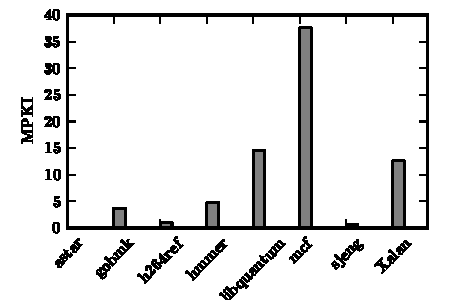
\includegraphics[width=3.46in]{figs/memstudy.pdf}
        \caption{Memory intensity of SPEC2006 benchmarks}
        \label{fig:memstudy}
    \end{center}
\end{figure}

The performance overhead results are shown in Figure~\ref{fig:performance}. The Y axis shows the total
execution time normalized to the baseline. As can be seen, the performance overhead is quite low
for the benchmarks with low memory intensity. For libquantum and mcf, the performance overhead is about 
25\%, which is still quite low compared to previous full system protection approaches which incurs serveral
times of overhead. The results show that our timing compartment architecture has moderate performance overhead
compared to an insecure architecture.

\begin{figure}
    \begin{center}
        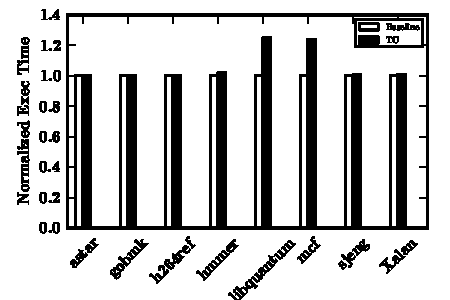
\includegraphics[width=3.46in]{figs/performance.pdf}
        \caption{Performance Overhead with 2 TCs}
        \label{fig:performance}
    \end{center}
\end{figure}

The performance overhead could get worse if the system scales up to more timing compartments. To give insight
about the performance overhead in terms of scaling, we evaluated the performance overhead with four timing
compartments, each occupying one core and private L1 and L2 caches. They share a 4MB L3 cache. The performance
overhead is shown in Figure~\ref{fig:scalability}. We show two bars for the baseline. One bar represents this
benchmark running with {astar, astar, astar}, and the other bar represents running with {mcf, mcf, mcf}. This
is because the baseline scheme shows different execution time when running with different benchmarks, and we
chose astar and mcf because they represents the least and most memory intensive benchmarks in our benchmark
suites. We also show the performance of our scheme. All the results are normalized to the baseline when running
with astar. Again, libquantum and mcf shows the highest overhead, 63\% and 79\% respectively, because of their 
high memory intensity. This overhead is still manageable compared to previous approaches.

\begin{figure}
    \begin{center}
        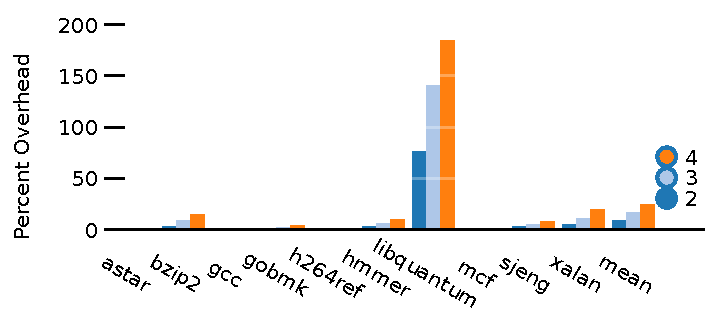
\includegraphics[width=3.46in]{figs/scalability.pdf}
        \caption{Performance Overhead with 4 TCs}
        \label{fig:scalability}
    \end{center}
\end{figure}


